\documentclass{standalone}
\usepackage[utf8]{inputenc}
\usepackage{tikz}
\usepackage{color}
\usetikzlibrary{arrows,shapes,positioning,shadows,trees}

\tikzset{
  basic/.style  = {draw, text width=3cm, drop shadow, font=\sffamily, rectangle},
  root/.style   = {basic, rounded corners=2pt, thin, align=center,
                   fill=red!60},
  level 2/.style = {basic, rounded corners=6pt, thin,align=center, fill=red!40,
                   text width=15em},
  level 3/.style = {basic, thin, align=left, fill=red!20, text width=10.1em}
}

\begin{document}

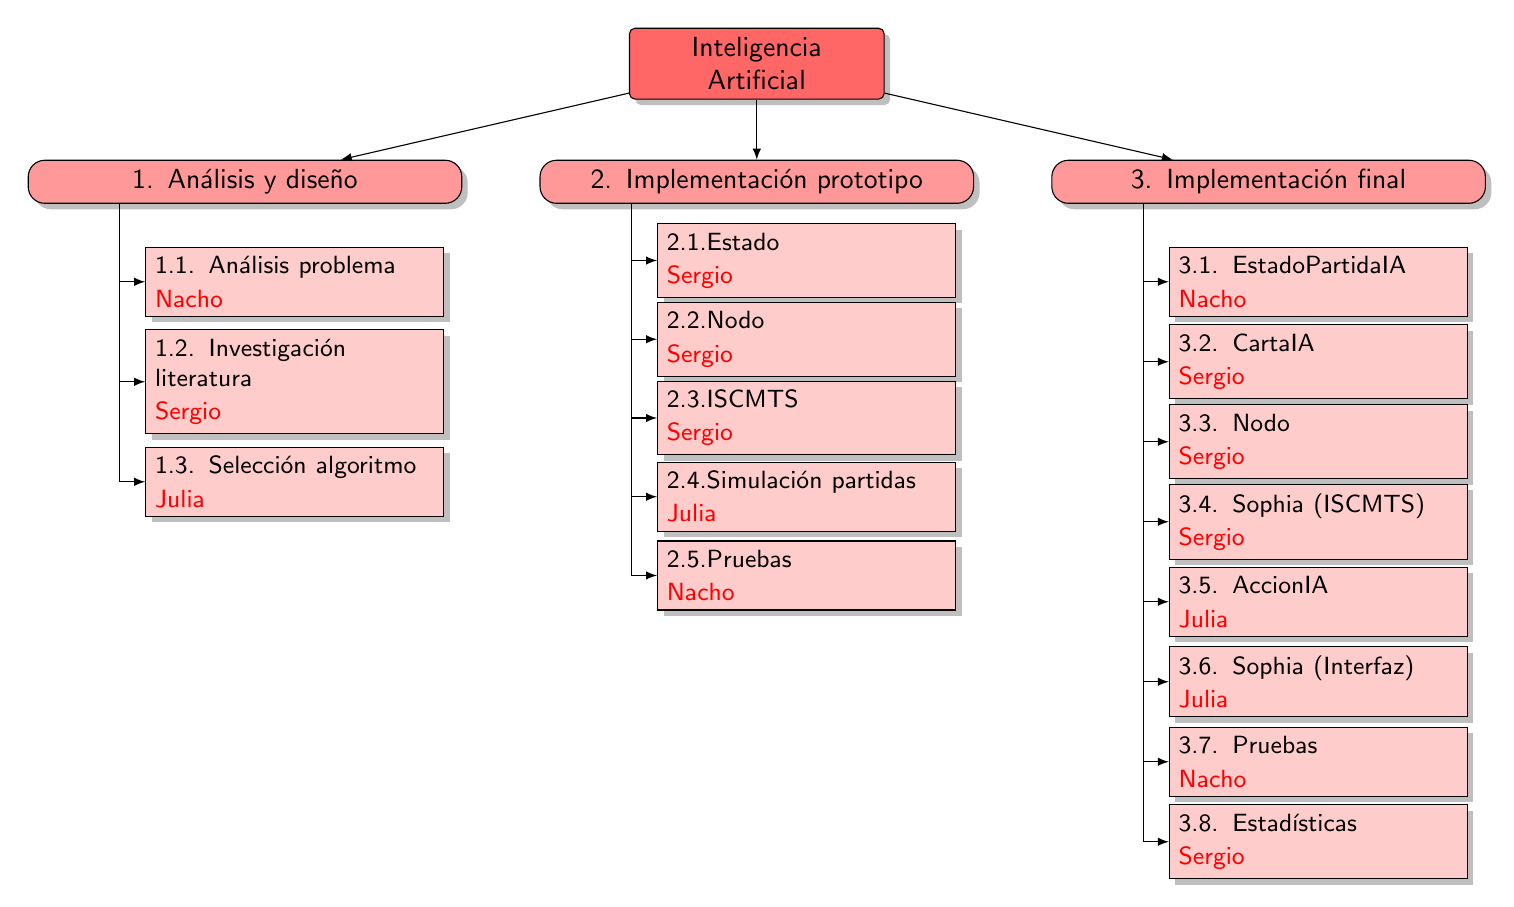
\begin{tikzpicture}[
  level 1/.style={sibling distance=65mm},
  edge from parent/.style={->,draw},
  >=latex]

% raiz inicial
\node[root] {Inteligencia Artificial}
% The first level, as children of the initial tree
  child {node[level 2] (c1) {1. Análisis y diseño}}
  child {node[level 2] (c2) {2. Implementación prototipo}}
  child {node[level 2] (c3) {3. Implementación final}};

% The second level, relatively positioned nodes
\begin{scope}[every node/.style={level 3}]
\node [below of = c1,node distance=0.5in, xshift=18pt] (c11) {\small{1.1. Análisis problema} \\ \textcolor{red}{\small{Nacho}}};
\node [below of = c11, node distance=0.5in] (c12) {\small{1.2. Investigación \\literatura}\\ \textcolor{red}{\small{Sergio}}};
\node [below of = c12, node distance=0.5in] (c13) {\small{1.3. Selección algoritmo} \\ \textcolor{red}{\small{Julia}}};

\node [below of = c2, xshift=18pt] (c21) {\small{2.1.Estado} \\ \textcolor{red}{\small{Sergio}}};
\node [below of = c21] (c22) {\small{2.2.Nodo} \\ \textcolor{red}{\small{Sergio}}};
\node [below of = c22] (c23) {\small{2.3.ISCMTS} \\ \textcolor{red}{\small{Sergio}}};
\node [below of = c23] (c24) {\small{2.4.Simulación partidas} \\ \textcolor{red}{\small{Julia}}};
\node [below of = c24] (c25) {\small{2.5.Pruebas} \\ \textcolor{red}{\small{Nacho}}};

\node [below of = c3, xshift=18pt, node distance = 0.5in] (c31) {\small{3.1. EstadoPartidaIA}\\ \textcolor{red}{\small{Nacho}}};
\node [below of = c31, node distance=0.4in] (c32) {\small{3.2. CartaIA}\\ \textcolor{red}{\small{Sergio}}};
\node [below of = c32, node distance=0.4in] (c33) {\small{3.3. Nodo}\\ \textcolor{red}{\small{Sergio}}};
\node [below of = c33, node distance=0.4in] (c34) {\small{3.4. Sophia (ISCMTS)}\\ \textcolor{red}{\small{Sergio}}};
\node [below of = c34, node distance=0.4in] (c35) {\small{3.5. AccionIA}\\ \textcolor{red}{\small{Julia}}};
\node [below of = c35, node distance=0.4in] (c36) {\small{3.6. Sophia (Interfaz)}\\ \textcolor{red}{\small{Julia}}};
\node [below of = c36, node distance=0.4in] (c37) {\small{3.7. Pruebas}\\ \textcolor{red}{\small{Nacho}}};
\node [below of = c37, node distance=0.4in] (c38) {\small{3.8. Estadísticas}\\ \textcolor{red}{\small{Sergio}}};
\end{scope}

\foreach \value in {1,...,3}
  \draw[->] (c1.190) |- (c1\value.west);

\foreach \value in {1,...,5}
  \draw[->] (c2.190) |- (c2\value.west);

\foreach \value in {1,...,8}
  \draw[->] (c3.190) |- (c3\value.west);
\end{tikzpicture}

\end{document}
